\documentclass[11pt,a4paper]{article}
\usepackage[margin=20mm]{geometry}
\usepackage{tikz}
\setlength{\parindent}{0pt}

\begin{document}
\begin{center}
  {\Large\bfseries BFS solution: exploration tree and frontier}
\end{center}
Start at $A$ in the undirected graph. Consider neighbors alphabetically; the
leftmost frontier vertex is next to be removed.

\vspace{5mm}
\textbf{Input graph}\par\vspace{2mm}
\begin{center}
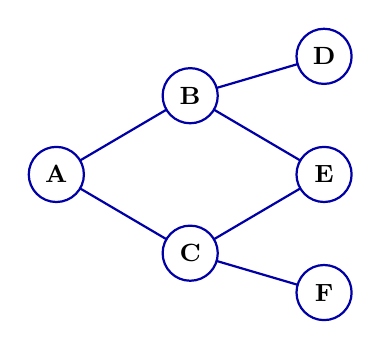
\begin{tikzpicture}[x=1cm,y=1cm]
  \draw[blue!65!black,thick] (0,0)--(1.7,1) (0,0)--(1.7,-1)
      (1.7,1)--(3.4,1.5) (1.7,1)--(3.4,0)
      (1.7,-1)--(3.4,0) (1.7,-1)--(3.4,-1.5);
  \tikzset{vertex/.style={circle,draw=blue!65!black,thick,fill=white,
          minimum size=7mm,inner sep=0pt,font=\small\bfseries}}
  \node[vertex] at (0,0) {A};
  \node[vertex] at (1.7,1) {B};
  \node[vertex] at (1.7,-1) {C};
  \node[vertex] at (3.4,1.5) {D};
  \node[vertex] at (3.4,0) {E};
  \node[vertex] at (3.4,-1.5) {F};
\end{tikzpicture}
\end{center}

\vspace{4mm}
\begin{center}
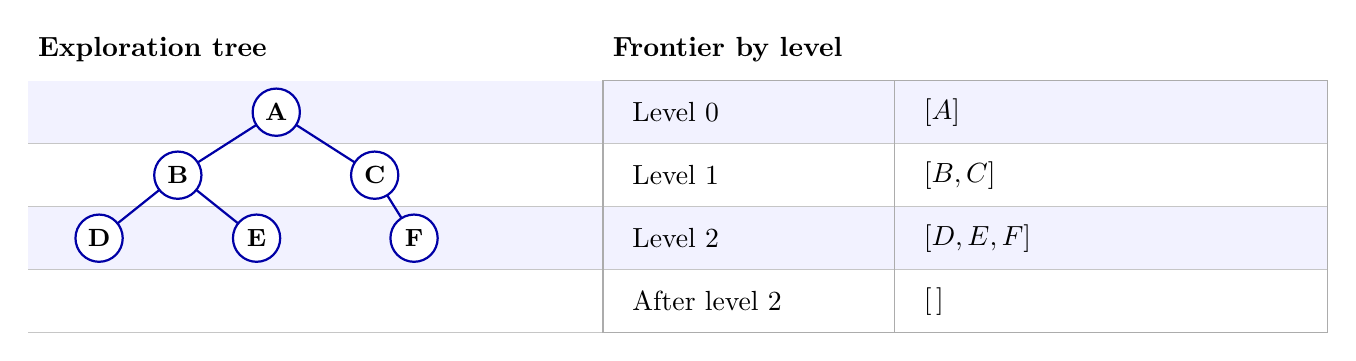
\begin{tikzpicture}[x=1cm,y=1cm]
  \fill[blue!5] (0,-0.5) rectangle (16.5,0.3);
  \fill[blue!5] (0,-2.1) rectangle (16.5,-1.3);
  \draw[gray!45] (0,-0.5)--(16.5,-0.5) (0,-1.3)--(16.5,-1.3)
                  (0,-2.1)--(16.5,-2.1) (0,-2.9)--(16.5,-2.9);
  \node[anchor=west,font=\bfseries] at (0,0.7) {Exploration tree};
  \node[anchor=west,font=\bfseries] at (7.3,0.7) {Frontier by level};

  % Row centers: -0.1, -0.9, -1.7, -2.5.
  \draw[gray!65] (7.3,0.3) rectangle (16.5,-2.9);
  \draw[gray!65] (11,-2.9)--(11,0.3);
  \node[anchor=west] at (7.55,-0.1) {Level 0};
  \node[anchor=west] at (11.25,-0.1) {$[A]$};
  \node[anchor=west] at (7.55,-0.9) {Level 1};
  \node[anchor=west] at (11.25,-0.9) {$[B,C]$};
  \node[anchor=west] at (7.55,-1.7) {Level 2};
  \node[anchor=west] at (11.25,-1.7) {$[D,E,F]$};
  \node[anchor=west] at (7.55,-2.5) {After level 2};
  \node[anchor=west] at (11.25,-2.5) {$[\,]$};

  \draw[blue!65!black,thick] (3.15,-0.1)--(1.9,-0.9)
      (3.15,-0.1)--(4.4,-0.9)
      (1.9,-0.9)--(0.9,-1.7)
      (1.9,-0.9)--(2.9,-1.7)
      (4.4,-0.9)--(4.9,-1.7);
  \tikzset{vertex/.style={circle,draw=blue!65!black,thick,fill=white,
          minimum size=6mm,inner sep=0pt,font=\small\bfseries}}
  \node[vertex] at (3.15,-0.1) {A};
  \node[vertex] at (1.9,-0.9) {B};
  \node[vertex] at (4.4,-0.9) {C};
  \node[vertex] at (0.9,-1.7) {D};
  \node[vertex] at (2.9,-1.7) {E};
  \node[vertex] at (4.9,-1.7) {F};
\end{tikzpicture}
\end{center}

\vspace{2mm}
$E$ was first discovered from $B$, so $C$--$E$ is not a tree edge.
\end{document}
